\chapter{Object Definition and Reconstruction}
\label{sec:obj}

\section{Tracks}
\label{sec:obj-tracks}

The ATLAS detector is able to reconstruct the trajectory of charged particles produced
in the proton-proton collision as they pass through the Inner Detector;
the reconstructed trajectories are known as tracks.
Track reconstruction is essential for a number of important areas of ATLAS analyses:
for example; primary vertex reconstruction, identification of $b$-hadrons (see Section~\ref{sec:obj-bjets})
and particle identification and measurement (such as the electrons and muons as described in Section~\ref{sec:obj-electron} and~\ref{sec:obj-muon}).

Track reconstruction uses hits from the Pixel detector, SCT and TRT which are described in Section~\ref{sec:det-ID}.
The track reconstruction is performed using an 'inside-out' approach,
which entails using the higher precision Pixel and SCT hits initially
and then adding in the TRT hits to improve track quality.
The tracking reconstruction procedure~\cite{obj-tracks_TIDE} follows these steps:
\vspace{-0.5em}
\begin{itemize}[leftmargin=*]
\item\textbf{Clustering:}
  \footnote{In the above reference this step is referred to as 'clusterization', which is not an actual word.}
  Neighbouring hits in a layer of the Pixel or SCT detector are converted into a 3D `space-point'
  that represents the point where the charged particle traversed the active material of the ID.
  In the Pixel detector one cluster of hits can form a space-point,
  whilst in the SCT hits from both sides of a strip layer are used to create a 3D space-point.\vspace{0.5em}
\item\textbf{Track Seeding:}
  Track seeds are formed from three space-points in consecutive layers of the Inner Detector
  that are consistent with the trajectory of a particle with $p_T >$ 500 MeV.\vspace{0.5em}
\item\textbf{Track Candidates:}
  From the track seeds, track candidates are built by iteratively adding space-points with a particle trajectory
  from the remaining Pixel and SCT detector layers using an combinatorial Kalman filter~\cite{obj-tracks_kal}.
  There can be multiple track candidates per seed.\vspace{0.5em}
\item\textbf{Track selection / Ambiguity resolving:}
  Each track is assigned a `track-score' that is based a number of variables of the track candidate;
  the $p_T$, $\eta$, $\chi^{2}$ fit and the hit pattern.
  Tracks must also pass some track quality requirements, that are again based on the track's $p_T$, $\eta$ and the hit pattern.
  The hit pattern refers to the number of Pixel or SCT hits,
  the number of holes (missing hits where one was expected)
  and the quality of the hits.
  The self-consistent set of tracks that have the highest `track-score' and that pass track quality requirements are then selected.
  Exact details of the track-scoring, track requirements and algorithm is described in~\cite{obj-tracks_TIDE}.\vspace{0.5em}
\item\textbf{Add TRT Information:}
  Tracks from the previous step are extrapolated into the TRT and all hits within \SI{10}{\milli\metre} are added.
  The tracks are then refitted using Pixel, SCT and TRT hits to make use of the full tracking detector.
\end{itemize}

The tracks resulting from the above track reconstruction process will be referred to as tracks in the remainder of this thesis.
Also it is important to note that, as discussed in Section~~\ref{sec:det-ID}, the tracks are curved by a known magnetic field in the Inner Detector,
therefore the tracks contain information on the charge and the momentum of the particles whose trajectory they are describing.

\section{Jets}
\label{sec:obj-jets}

If a collision results in a free quark or gluon in its final state then a stream of high-energy hadrons is created,
which is known as a hadronic jet.
The underlying processes in hadronic jet formation can be summarised as follows;
firstly the free quark/gluon will radiate additional gluons and quarks in a process known as the parton shower,
these gluons and quarks will then undergo hadronisation to form hadrons which are the constituents of the hadronic jet.
A more detailed description of the parton shower and hadronisation process can be found in Section~\textit{[QCD theory description] Not written yet} \textbf{LM fix}.
The components of the hadronic jet deposit energy in the cells of the ATLAS calorimeter, through the processes described in Section~\ref{sec:det-calo},
such that the ATLAS calorimeter has an energy measurement of the components of the hadronic jet, within the spatial limits from the granularity of the detector.
The process of parton shower, hadronisation and energy deposition in the calorimeter  described above is illustrated in Figure~\ref{fig:obj-jets_schem}.

\begin{figure}[!ht]
  \begin{center}
    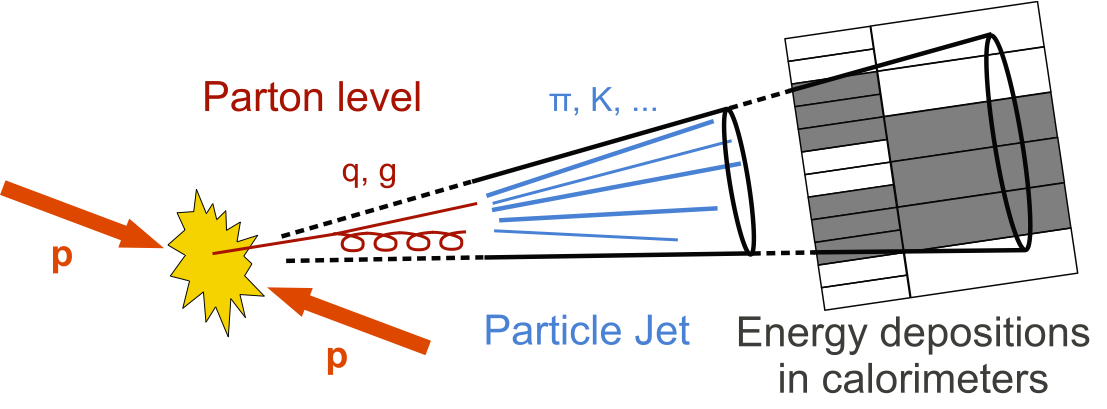
\includegraphics[width=0.8\linewidth, angle=0]{figs/Objects/jets_schem.png}
  \end{center}
  \caption[A schematic illustrating the formation of hadronic jets and the resulting observed energy deposits in the calorimeter system.]
          {A schematic illustrating the formation of hadronic jets and the resulting observed energy deposits in the calorimeter system \cite{obj-jets_schem}.}
  \label{fig:obj-jets_schem}
\end{figure}

This section contains a description of the procedure utilised by ATLAS
to go from energy deposits in calorimeter cells to well defined and calibrated hadronic jets.
This procedure can be split up into three separate steps that are described in the following sections;
firstly topoclusters are formed as described in Section~\ref{sec:obj-jets_topo},
then jets are formed from topoclusters using reclustering algorithms described in Section~\ref{sec:obj-jets_reco}
and finally Section~\ref{sec:obj-jets_reco} describes how the jets are calibrated and the relevant jet energy uncertainties are derived.

In this section the formation of hadronic jets constructed from calorimeter cells is described,
as this is the only jet object used in the context of the analyses presented in this thesis.
However, it is worth noting, that there are other types of jets used at ATLAS;
jets are used to observe electrons and taus whilst
hadronic jets can also be constructed from tracks formed in the Inner Detector, a technique that has been useful in dense environments~\cite{obj-Hbb}.

\subsection{Hadronic Topocluster Reconstruction}
\label{sec:obj-jets_topo}

The first step of jet building at ATLAS is the formation of 3D clusters, known as topoclusters, from groups of energy deposits in neighbouring calorimeter cells~\cite{obj-jets_topo}.
The calorimeter cells can be from either the EM or hadronic calorimeter systems,
which have a granularity given in Table~\ref{tab:det-calo_granularity}.
The algorithm employed makes use of the variable ``cell signal significance'' defined as, 
\begin{equation}
  \Large{S_{\text{cell}} = \frac{E_{\text{cell}}}{\sigma_{\text{noise,cell}}}}
\end{equation}
where $E_{\text{cell}}$ is the energy deposited in a cell
and $\sigma_{\text{noise,cell}}$ is the uncertainty due to noise in that cell.
The sources of noise in a calorimeter cell are described in Section \textbf{LM fix, need to have a noise section somewhere...}.
A large value of $S_{\text{cell}}$ ( $>$ 1 ) indicates that the energy deposit is likely due to a particle
depositing energy in the calorimeter rather than noise within the calorimeter.

\noindent
Using the value of $S_{\text{cell}}$, each calorimeter cell is labelled as follows
\begin{itemize}
\item If $|S_{\text{cell}}| > 4$: the cell is labelled a \textbf{seed} cell.
\item If $|S_{\text{cell}}| > 2$: the cell is labelled a \textbf{growth} cell.
\item If $|S_{\text{cell}}| > 0$: the cell is labelled a \textbf{boundary} cell.
\end{itemize}
Then the algorithms builds topoclusters as in the following steps,
\begin{enumerate}
\item A seed cell forms the centre of a new topocluster.
\item Neighbouring seed cells are added together to form one topocluster seed.
\item Then, growth cells neighbouring the topocluster are added.
\item Finally, boundary cells neighbouring the topocluster are added.
\end{enumerate}
Figure~\ref{fig:obj-topo_schem} illustrates an example of where the algorithm would form a topocluster and an example where it wouldn't.

The topoclusters are treated as massless objects,
such that the four-momentum of each deposit can be calculated using the sum of energy deposited in the topoclusters
and the $\eta-\phi$ position of the topocluster.
The constructed topoclusters and their four-momentums are then used as the inputs to the next step of jet reconstruction.

\begin{figure}[!hbt]
  \begin{center}
    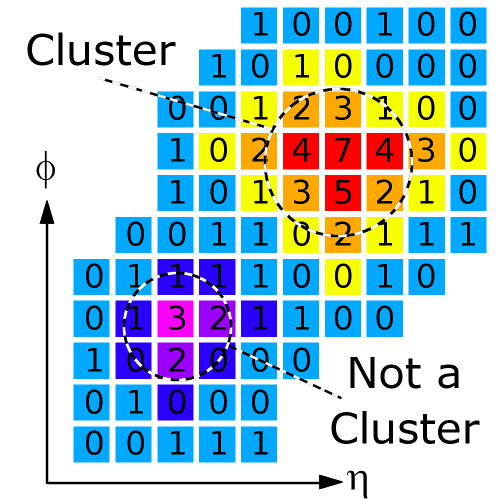
\includegraphics[width=0.7\linewidth, angle=0]{figs/Objects/topo_schem.png}
  \end{center}
  \caption[A schematic illustrating the algorithm used to form a topocluster. The numbers on the grid represent $|S_{\text{cell}}|$ and the colours represent the cell label.]
          {A schematic illustrating the algorithm used to form a topocluster. The numbers on the grid represent $|S_{\text{cell}}|$ and the colours represent the cell label~\cite{det-magnet_fig}.}
  \label{fig:obj-topo_schem}
\end{figure}

\FloatBarrier
\newpage
\subsection{Jet Reconstruction}
\label{sec:obj-jets_reco}

The next step in the process is to form jets from the topoclusters described in the previous section.
To do this a jet reconstruction algorithm is defined, that uses the spatial and energy information of the topoclusters in an event
to form a set of jets.
Each jet formed by the algorithm has a well defined four-momentum and set of constituents.
Jet reconstruction algorithms are used to define jets as this means that jets are experimentally well-defined model-independent observables,
which is required if measurements using jets are to be re-usable by the wider particle physics community.
A detailed discussion of jet reconstruction algorithms
and their related issues is found in~\cite{obj-jets_reco_salam};
as such this section provides a summary relevant to the analyses being presented in this thesis.

ATLAS analyses use a type of jet reconstruction algorithms known as sequential recombination algorithms,
which selectively add together the calorimeter topoclusters to form the jet;
these are specifically the $k_t$, anti-$k_t$ and Cambridge-Aachen (CA) algorithms.

The three algorithms use a set of four-momentums (clusters), which are initially the topoclusters formed in the calorimeter.
One then introduces an inter-jet distance between clusters $i$ and $j$ defined as,
\begin{equation}
  d_{ij} = \text{min}
  [(p_{ Ti})^a, (p_{ Tj})^a]  \left(\frac{\Delta  R_{ij}}{R}\right) ^2, \hspace{1cm} \Delta R_{ij} = \sqrt{(y_{i} - y_{j})^2 + (\phi_{i} - \phi_{j})^2} \label{dij}
\end{equation}
\noindent and a particle-beam distance for cluster $i$ defined as,
\begin{equation}
  d_{iB} = (p_{Ti})^a \label{diB}
\end{equation}
where $y$  is rapidity (as defined in Section~\ref{sec:det-coordinate}), $\phi$ is azimuthal angle,
$p_T$ is transverse momentum (component of momentum perpendicular to the beam-pipe of colliding particles)
and $p_z$ is the component of momentum that is parallel to the beam-pipe of colliding particles.
$R$ is the jet width parameter, a free parameter of the algorithm.
The parameter $a$ in Eq. \eqref{dij} and \eqref{diB} takes the value $a = 2$ for the $k_t$ algorithm, $a = -2$ for the anti-$k_t$ algorithm 
and  $a = 0$ for the Cambridge-Aachen algorithm.

The inter-jet and particle-beam distances are not physical distances as such, but can instead be thought of as dimensionful measures of how likely it is that
clusters $i$ and $j$ represent clusters caused by hadrons from the same jet.
If the inter-jet distance for a pair of clusters is smaller than the particle-beam distances for the two clusters ($d_{ij} < d_{iB}$) 
then it is likely that the two clusters are from the same jet. 
In contrast, if $d_{ij} > d_{iB}$ then it is unlikely that the two clusters are from the same jet.
 
\noindent The algorithm then proceeds using the following steps:
\vspace{-1em}
\begin{enumerate}[nolistsep]
  \item Calculate $d_{ij}$ and $d_{iB}$ for all combinations of clusters.  
  \item Find the minimum of the $d_{ij}$ and $d_{iB}$. 
  \item If the minimum is a $d_{ij}$ combine cluster $i$ and $j$ to form a new cluster and return to step 1. 
  \item If the minimum is a $d_{iB}$ then call cluster $i$ a final-state jet, remove it from the set and return to step 1.  
  \item Stop when all clusters have been declared as jets. 
\end{enumerate} 
The final jet has a four-momentum equal to the addition of all the topoclusters assigned to that jet.
It can now be seen that the jet width parameter, $R$, effectively gives the scale of the width of a reconstructed jet.
This is because when $\Delta R_{ij} > R$ for a pair of clusters,
$d_{iB} < d_{ij}$ for the cluster with the smaller value of ${p_T}$,
and thus the algorithm will not merge the two clusters.

The sequential reclustering algorithms described above are used as they satisfy two important theoretically motivated criteria:
infrared and collinear safety.
Infrared safety requires that the jet reconstruction algorithm result should be invariant against soft gluon emission \footnote{Soft means a low momentum}
and collinear safety requires that the jet reconstruction algorithm result should be invariant against a parton splitting into two partons with small angular separation.
These conditions are desirable as if the jet reconstruction algorithm is infrared or collinear unsafe,
two identical hard-scatter processes could be observed entirely differently due to an additional emission process in the parton shower or hadronisation process.
The sequential reclustering algorithms described above are infrared and collinear safe.
\footnote{Cone-based algorithms jet reconstruction algorithms used at some previous collider experiments,
  such as UA2 ~\cite{obj-jets_reco_UA2}, do not satisfy this infrared and collinear safety.}.

Anti-$k_T$ is the jet reconstruction algorithm used for the analyses being presented in this thesis, which is typical of analyses at ATLAS.
This is because the anti-$k_T$ algorithm provides regular jet shapes around the centre of the jet,
due to the fact that the algorithm reconstructs the high-$p_T$ core of the jets first and then adds in the lower $p_T$ suburbs in later steps.
Figure~\ref{fig:obj-jets_reco_shapes} shows the jets formed by the Cambridge-Aachen, $k_T$ and anti-$k_T$ algorithm using the same set of input clusters;
this illustrates that anti-$k_T$ algorithm creates more regular jet shapes than the other sequential-reclustering algorithms.
Further to this, the value of the jet width parameter is chosen as $R$=0.4, which is the standard value used in ATLAS analyses.
\textbf{LM: I think this part needs a bit more on why R=0.4}

\begin{figure}[!ht]
  \captionsetup[subfigure]{aboveskip=-5pt,justification=centering}
  \begin{center}
    \subcaptionbox{Cambridge-Aachen} {
      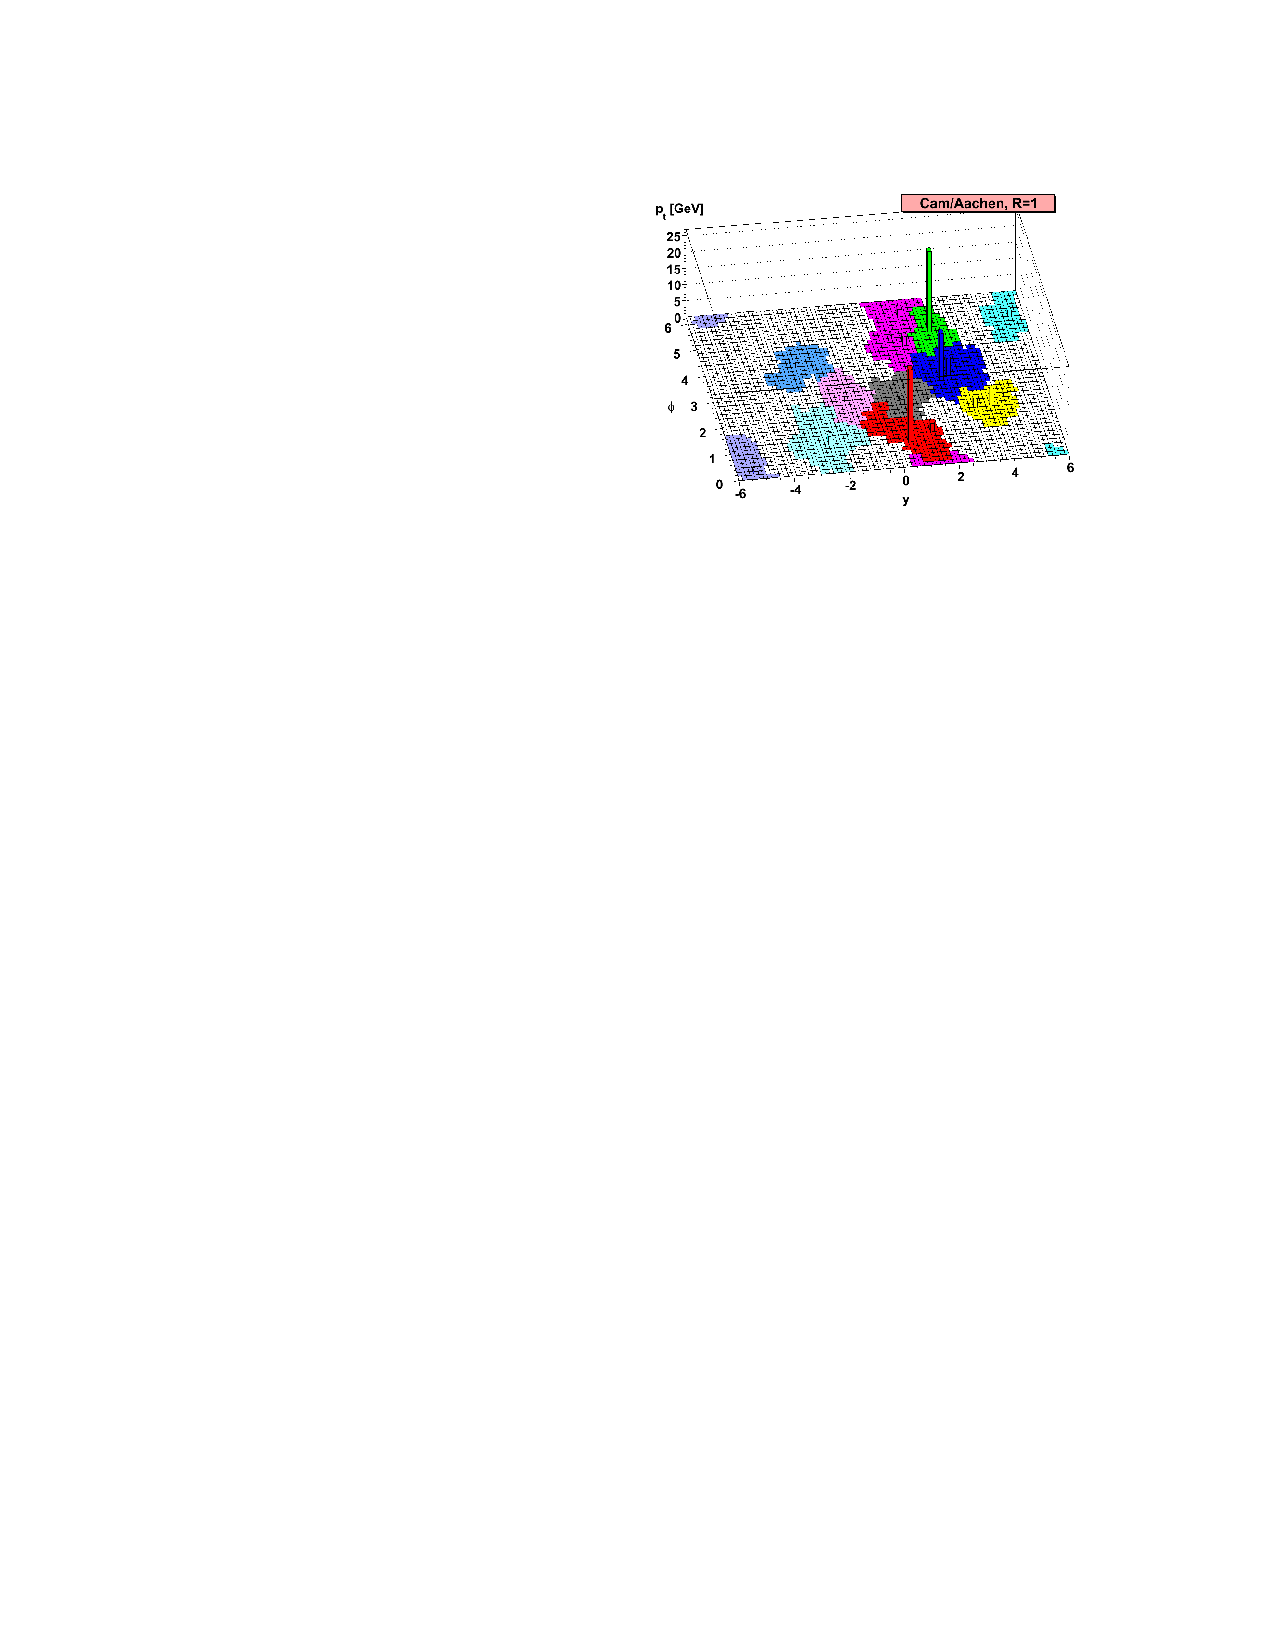
\includegraphics[width=0.45\linewidth, angle=0]{figs/Objects/jets_reco_shapes_ca.pdf}
    }
    \subcaptionbox{$k_T$} {
      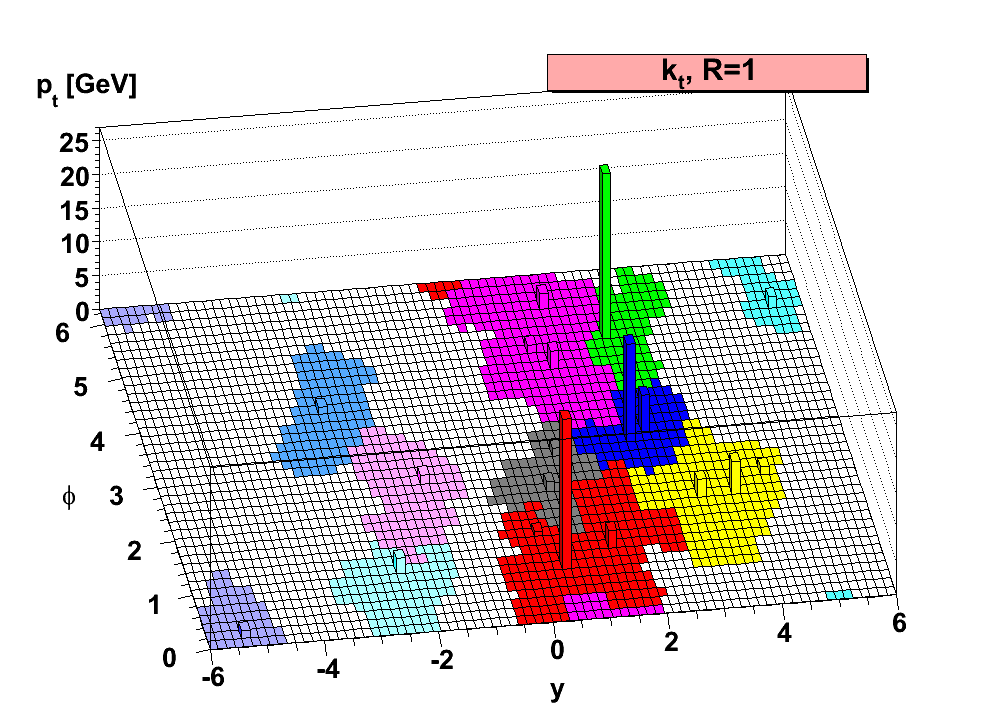
\includegraphics[width=0.45\linewidth, angle=0]{figs/Objects/jets_reco_shapes_kt.png}
    }\\
    \subcaptionbox{Anti-$k_T$} {
      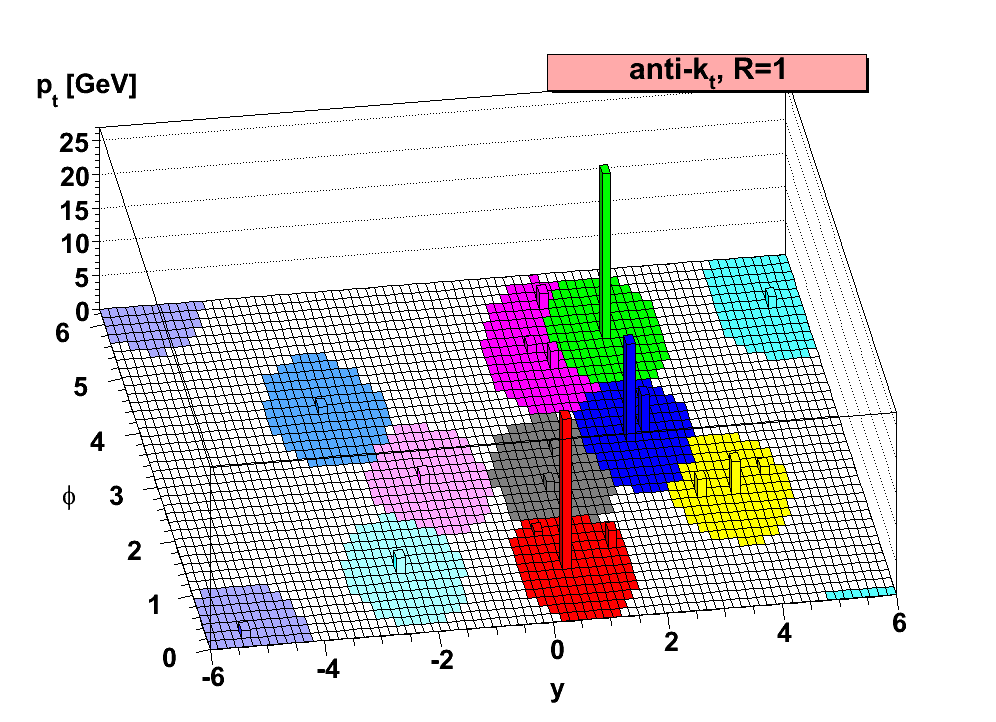
\includegraphics[width=0.45\linewidth, angle=0]{figs/Objects/jets_reco_shapes_akt.png}
    }

  \end{center}
  \caption[A comparison of the jets formed using the (a) Cambridge-Aachen, (b) $k_T$ and (c) anti-$k_T$ algorithm from the same simulated event.
    The constituent clusters of each of the jets formed is indicated using various colours.]
          {A comparison of the jets formed using the (a) Cambridge-Aachen, (b) $k_T$ and (c) anti-$k_T$ algorithm from the same simulated event.
            The constituent clusters of each of the jets formed is indicated using various colours \cite{obj-jets_reco_akt}.}
  \label{fig:obj-jets_reco_shapes}
\end{figure}

\subsection{Jet Calibration}
\label{sec:obj-jets_calib}

The jets initially formed by the jet reclustering algorithms from the topoclusters
will not represent the energy of the initial parton
and as such will not give an accurate dijet mass reconstruction which is required for the analyses presented in this thesis.
As a result, a hadronic jet calibration is required to map the initial reconstructed jet
to a more representative calibrated jet that can be used in an analysis.

\noindent
The key factors for the unrepresentative hadronic jet energy measurement are~\cite{det-thesis_kate,obj-bjets_algo_2015}:
\begin{itemize}[leftmargin=*]
\item\textbf{Jet energy scale}:
  As discussed in Section~\ref{sec:det-calo_HCAL}, the ATLAS calorimeter is non-compensating which means that
  the calorimeter response is different for an EM-object and a hadronic object.
  The calorimeter response is calibrated at the EM-scale such that the energy measurements from a calorimeter cell
  are correct for an EM-object;
  as a result the initial energy measurement for a hadronic jet will be incorrect.
  To account for this a correction is required to take the jet energy measurement from the EM-scale to the hadronic-scale.\vspace{0.5em}
\item\textbf{Dead Material}:
  The hadronic jet may overlap with an unresponsive region of the detector,
  resulting in some energy deposits being incorrectly measured.\vspace{0.5em}
\item\textbf{Leakage}:
  Some energy from the jet will be distributed outside the angular acceptance of the calorimeter
  whilst some energy will pass through the calorimeter in a process known as `punch-through', as discussed in Section~\ref{sec:det-MS}.\vspace{0.5em}
\item\textbf{Reconstruction Issues}:
  There are two issues with jet reconstruction that require correction:
  firstly, some energy deposits coming from the initial parton may not be constructed as topoclusters due to the cell signal significance thresholds required in topocluster formation.
  Secondly, some topoclusters that should be clustered to the jet may not included in the reconstructed jet or included in a different jet instead.\vspace{0.5em}
\item\textbf{Pile-up}:
  Energy from collisions other than the hard-scatter collision can also be included by the reclustering algorithm.
  This includes in-time and out-of-time pile-up.
  A  definition of pile-up can be found in Section~\cite{}. \textbf{LM Fix: Need a description of pile-up, probably in LHC running conditions}
\end{itemize}

As a result of the factors listed above a correction to the jets must be applied;
which is done using the procedure described in~\cite{obj-jets_calib_run2}.
An executive summary of the procedure is found below.

An important input of applying a calibration is deciding what one is correcting with respect to.
The truth initial parton seems at first like a good choice,
however this correction depends strongly on the theoretical modelling of the parton shower and hadronisation process,
hence, this would mean that the calibrated jets are not model-independent.
Instead, in ATLAS jets are corrected with respect to a `truth jet';
where a truth jet is defined as a jet formed in a simulated event from running the anti-$k_T$ algorithm on the set of stable truth particles in a simulated event.
A stable particle is required to have a lifetime $c\tau >$ \SI{10}{\milli\metre} and muons, neutrinos, and particles from pile-up collisions are ignored.
Truth jets are well-defined and model-independent objects representing the jets that would have been reconstructed if one had a perfect detector;
therefore they are a good choice for jet corrections.

The calibration process uses Monte-Carlo simulation and data to correct reconstructed jets to data using a number of steps;
starting from the initially formed EM-scale jets.
These steps are outlined in Figure~\ref{fig:obj-jets_calib_schem}.

\begin{figure}[!htb]
  \begin{center}
    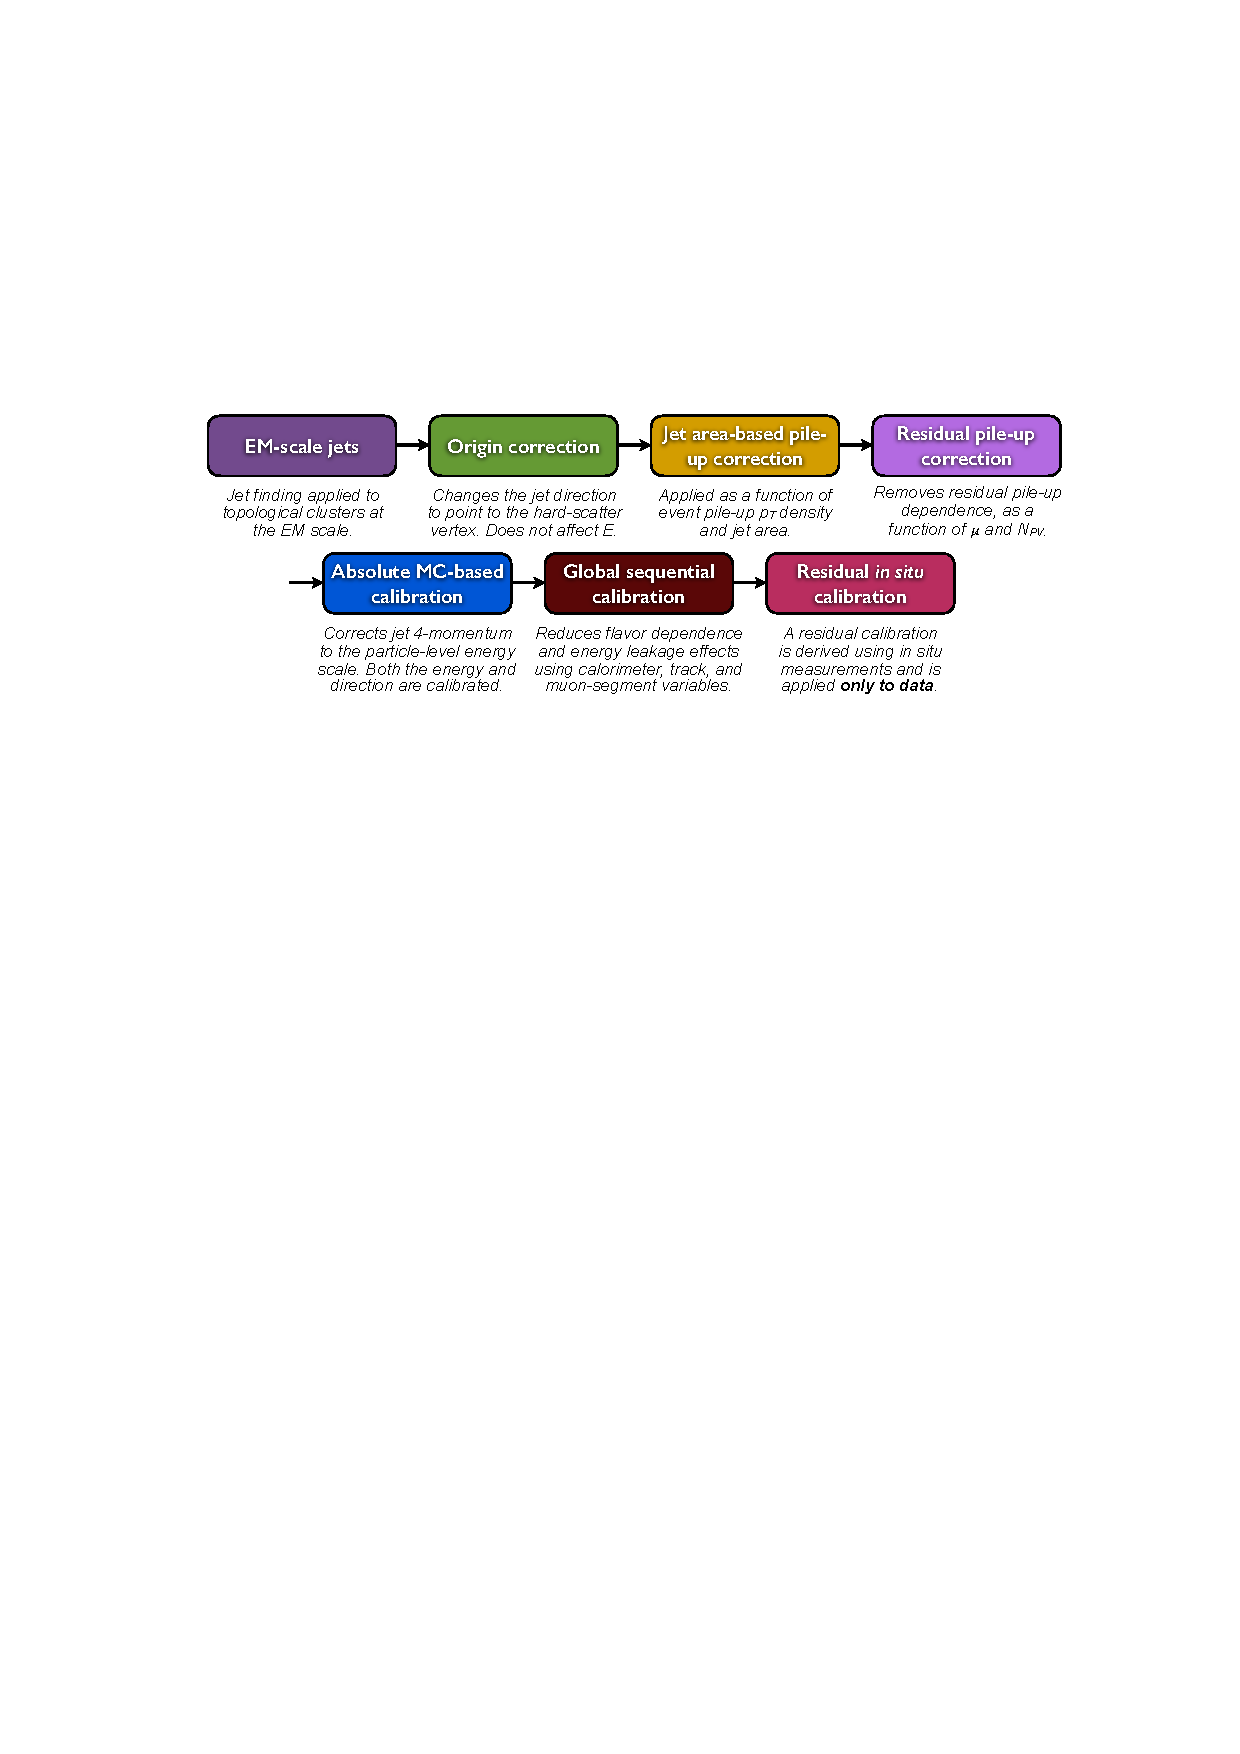
\includegraphics[width=0.9\textwidth]{figs/Objects/jets_calib_schem.pdf}
    \caption[Calibration stages for EM-scale jets. Other than the origin correction, each stage of the calibration is applied to the four-momentum of the jet.]
            {Calibration stages for EM-scale jets. Other than the origin correction, each stage of the calibration is applied to the four-momentum of the jet~\cite{obj-jets_calib_run2}}
    \label{fig:obj-jets_calib_schem}
  \end{center}
  \vspace{-0.5cm}
\end{figure}

\noindent
To discuss each step in a little more detail:
\begin{itemize}[leftmargin=*]
\item\textbf{Origin Correction}:
  This step changes the direction of the jets such that the four-momentum points to the hard-scatter primary vertex
  rather than the centre of the detector.
  This calculation conserves the jet energy.\vspace{0.5em}
\item\textbf{Jet Area-Based Pile-up Correction}:
  This step removes unwanted energy contributions from pile-up.
  This correction subtracts the area of the jet, $A$, multiplied by the average energy density due to pile-up, $\rho$.\vspace{0.5em}
\item\textbf{Residual Pile-up Correction}:
  This step further reduces effects from pile-up utilising the linear dependence of pile-up effects on
  the number of primary verticies, $N_{PV}$
  and the mean number of additional $pp$ collisions per bunch crossing of the event, $\mu$.\vspace{0.5em}
\item\textbf{Absolute JES Correction}:
  This step corrects the jet four-momentum from the EM-scale, at which they were initially formed,
  to the hadronic-scale, which is defined in terms of the truth jets in simulation.
  This correction is derived using truth jets and reconstructed detector-level jets in dijet Monte-Carlo events.\vspace{0.5em}
\item\textbf{Global Sequential Calibration}:
  This step uses information from the calorimeter, muon spectrometer and track-based variables
  to reduce the reconstructed energy and the reduce the overall uncertainties\footnote{Jet energy uncertainties are discussed in the next Section~\ref{sec:obj-jets_uncert}.}.\vspace{0.5em}
\item\textbf{In-situ calibration}:
  All previous steps in this calibration have been done using simulation to correct
  detector-level jets to truth jets. This step accounts for any differences between simulation and data.
  This step uses events containing a jet to be calibrated and a well-measured reference objects, including photons, Z bosons, and calibrated jets.
  Then conservation of momentum gives us information on the true $p_T$ of the jet to be calibrated.
  One can calculate a double ratio with respect to jet-$p_T$;
  \begin{equation}
    \text{Correction} = \frac{1}{R(p_T, \eta)} = \frac{ < p_T^{\text{jet}}/p_T^{\text{ref}}>_{\text{MC}} }{ < p_T^{\text{jet}}/p_T^{\text{ref}}>_{\text{Data}} }
  \end{equation}
  which is applied as a correction to jet $p_T$ in data; this correction is not applied in simulation.
\end{itemize}

A jet formed by this calibration scheme is known as an EM-Topo jet, as the topoclusters are at the EM-scale.
Here, I should note that there are other schemes used for calibrating jets at ATLAS,
for example some analyses~\cite{obj-VVjj} correct each topocluster to the hadronic scale
before clustering the jet, in a scheme called Local Cluster Weighted (LCW)~\cite{obj-jets_topo}.
\textbf{LM Fix, why use EM-Topo, smaller errors...}

The end result of the processes described in this section is a jet,
reconstructed from EM-scale topoclusters using an anti-$k_T$ algorithm with a jet width parameter $R$=0.4,
which has been calibrated using simulation and an data-driven in-situ step.
The result of this process is what is known as an anti-$k_T$ R=0.4 EM-Topo jet,
and is the definition for a jet in this thesis.

\subsection{Jet Energy Uncertainties}
\label{sec:obj-jets_uncert}

All measurements have uncertainties, and this section investigates the uncertainties of jet energy measurement.
Jet energy measurements separate the associated uncertainties into two components;
jet energy resolution and jet energy scale.

Jet energy resolution (JER) is defined as $\sigma(E)/E$, and JER uncertainties
come from an imperfect simulation of detector resolution in Monte-Carlo simulation.
This uncertainty is measured using an in-situ technique from the balancing of jets in 8 TeV collision data
which is extrapolated for 13 TeV data; the final uncertainty accounts for this extrapolation.
Figure~\ref{fig:obj-jets_calib_JER} shows the fractional JER uncertainty as a function of jet-$p_T$ and jet-$\eta$.
Full details on the derivation of this uncertainty can be found in~\cite{obj-jets_calib_2015}~and~\cite{obj-jets_calib_JER_8TeV}.

\begin{figure}[!ht]
  \begin{center}
    \captionsetup[subfigure]{aboveskip=0pt,justification=centering}
    \subcaptionbox{Jet-\pT} {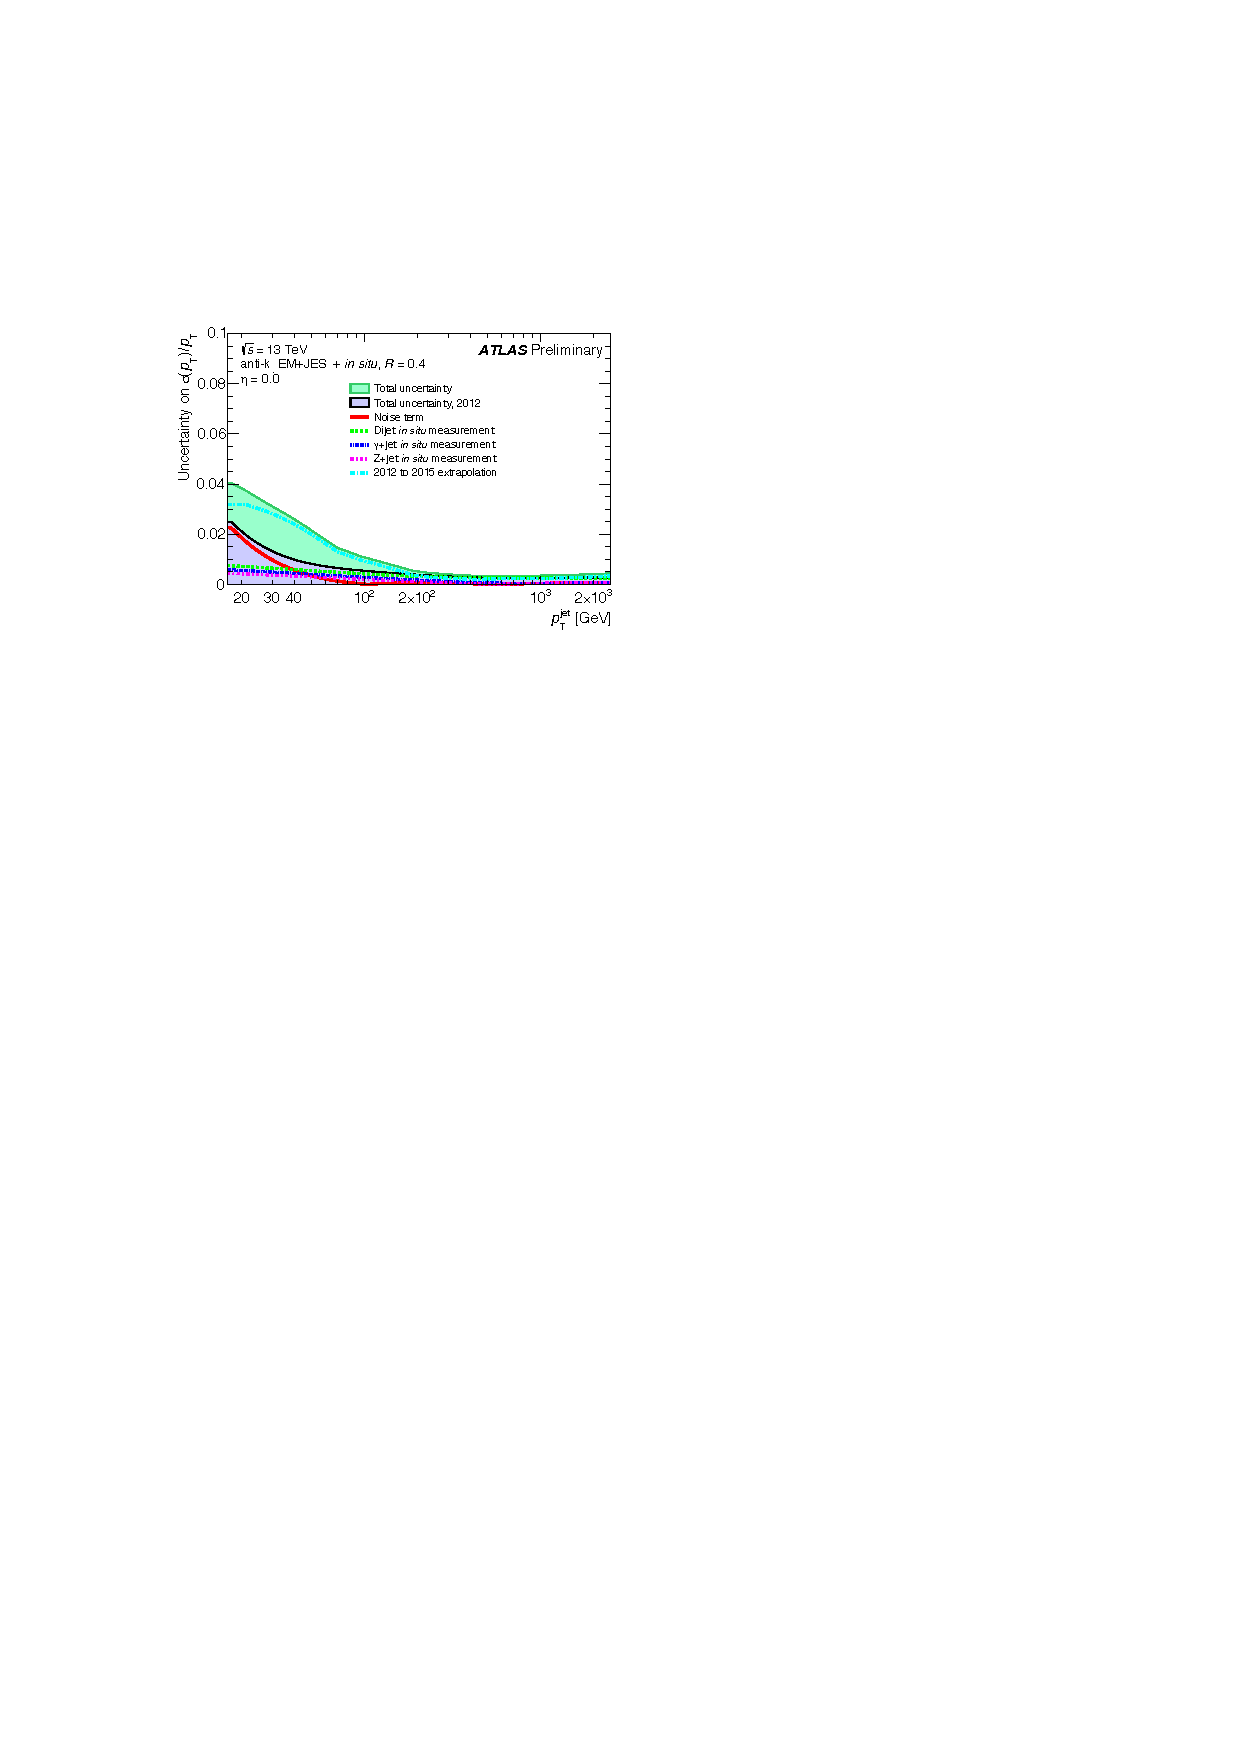
\includegraphics[width=0.48\linewidth, angle=0]{figs/Objects/jets_uncert_JER_pt.pdf} }
    \subcaptionbox{Jet-\eta}{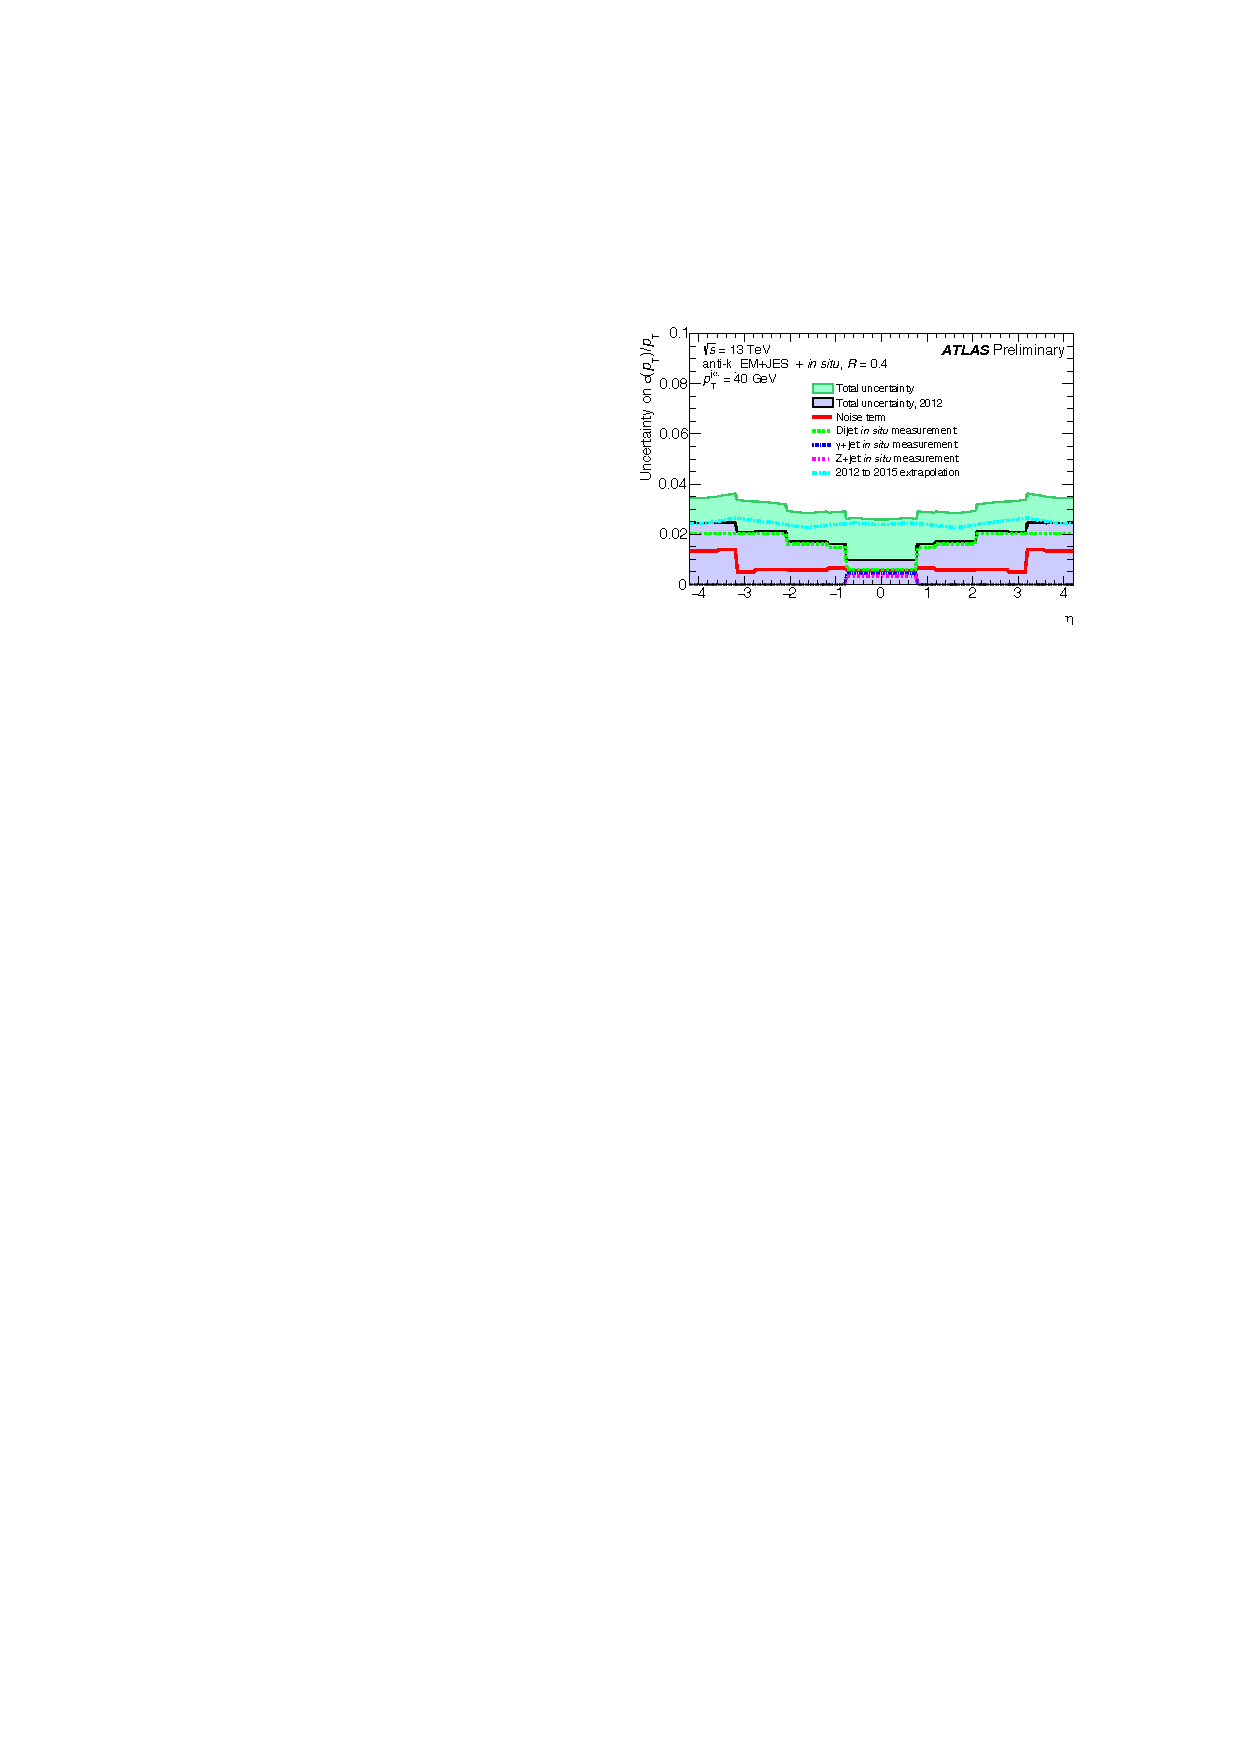
\includegraphics[width=0.48\linewidth, angle=0]{figs/Objects/jets_uncert_JER_eta.pdf} }
  \end{center}
  \caption[The fractional jet energy resolution uncertainty as a function of jet-\pT and \eta.
    The total uncertainty is shown as are the contributions from the various sources of uncertainty.]
          {The fractional jet energy resolution uncertainty as a function of jet-\pT and \eta.
            The total uncertainty is shown as are the contributions from the various sources of uncertainty ~\cite{obj-jets_calib_2015}.}
  \label{fig:obj-jets_calib_JER}
\end{figure}

Jet energy scale (JES) uncertainties arise from the calibration procedure
to correct jets from the EM-scale to the hadronic-scale, outline above.
80 separate uncertainties are derived to cover each step of the calibration.
Figure~\ref{fig:obj-jets_calib_JES} shows the fractional JES uncertainty as a function of jet-$p_T$ and jet-$\eta$.
Full details on the uncertainty derivation can be found in~\cite{obj-jets_calib_run2}.

\begin{figure}[!ht]
  \begin{center}
    \captionsetup[subfigure]{aboveskip=0pt,justification=centering}
    \subcaptionbox{Jet-\pT} {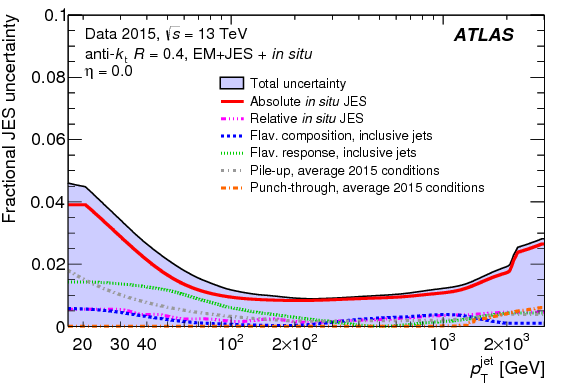
\includegraphics[width=0.48\linewidth, angle=0]{figs/Objects/jets_uncert_JES_pt.png} }
    \subcaptionbox{Jet-\eta}{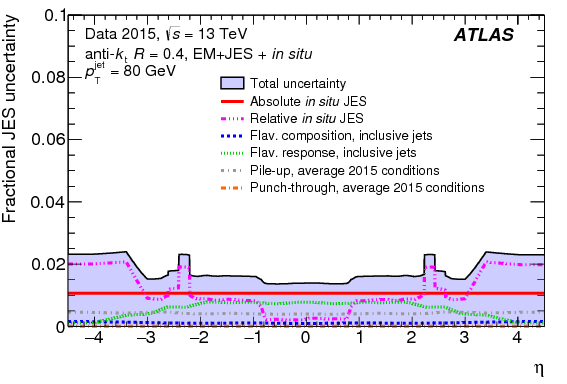
\includegraphics[width=0.48\linewidth, angle=0]{figs/Objects/jets_uncert_JES_eta.png} }
  \end{center}
  \caption[The fractional jet energy scale uncertainty as a function of jet-\pT and \eta.
    The total uncertainty is shown as are the contributions from the various sources of uncertainty.]
          {The fractional jet energy scale uncertainty as a function of jet-\pT and \eta.
            The total uncertainty is shown as are the contributions from the various sources of uncertainty ~\cite{obj-jets_calib_run2}.}
  \label{fig:obj-jets_calib_JES}
\end{figure}

\FloatBarrier

\newpage
\section{Identification of $b$-jets}
\label{sec:obj-bjets}

Hadronic jets, described in Section~\ref{sec:obj-jets}, can be further categorised into three separate categories based on the flavour of the constituent quarks.
$b$-jets are defined as jets containing one or more $b$-hadrons,
$c$-jets are defined as jets containing one or more $c$-hadrons but no $b$-hadrons
and finally light-flavoured jets comprise of only light hadrons (\textit{u}, \textit{d} and \textit{s} quarks).
A description of how this definition is practically used in simulation is given in Section~\ref{sec:obj-bjets_label}.

The identification $b$-jets, known as $b$-tagging, has been an essential tool in a range of ATLAS collaboration results;
for example analyses studying the $t\bar{t}$ final state \cite{obj-ttbar} \footnote{Section~\ref{sec:trig-bjet_eff} contains a concrete example of this.}
and the first direct evidence of the Higgs boson coupling to the quark-sector~\cite{obj-Hbb}.
%In the former, as the top decays to a \textit{W}-boson and a $b$-quark with a branching ratio close to 100\%, 
%the application of $b$-tagging can be used increase purity, this is used in the study described in Section~\ref{sec:trig-sys}.
%In the latter, the Higgs boson coupling is proportional to mass squared, hence the large mass of the
%$b$-quark means that $H\to b\bar{b}$ is the decay of the Higgs boson with the largest branching-ratio
%which means that it is the best channel to make the first direct observation of the Higgs boson coupling to fermions.
In the same sense, identification of $b$-jets is an essential part of the analysis being presented here;
by selecting $b$-jets we increase our sensitivity to BSM models that decay to 1 or 2 $b$-jets in their final state.
\textbf{Laurie Fix, link to where I explain why this is good, maybe Intro}.

The process of $b$-tagging at ATLAS in Run-2 has been previously described in great
detail~\cite{obj-bjets_algo_2015,obj-bjets_algo_2016},
so what follows is a summary of the key features of the process.

\subsection{Assigning a Flavour Label}
\label{sec:obj-bjets_label}

In simulation, the particle-level truth information is known, and hence a truth flavour label of a jet can be defined.
Flavour is assigned to jets by matching truth-level heavy-hadrons with $p_{T} >$ 5 GeV and $\Delta R <$ 0.3 between the hadron and the jet.
If a $b$-hadron is matched to a jet, the jet is then declared a $b$-jet;
this process is then repeated for $c$-hadrons and then $\tau$ leptons.
If no match between $b$, $c$ or $\tau$ is achieved then the jet is assigned as a light-flavour jet.
The matching is exclusive, which means that each particle is only assigned to one jet. \textbf{Add a reference, possibly performance}
This definition of truth flavour in simulation is used generally within this thesis.
   
\subsection{Algorithm descriptions}

To identify $b$-jets, $b$-tagging algorithms utilise the long lifetimes of the heavy-hadrons that decay through the flavour changing weak interaction,
a hadron containing a $b$-quark has a lifetime of the order \SI{1.5}{\pico\second} %\cite{obj-bjets_algo_2015}.
A $b$-jet decay chain  will typically contain two of these flavour changing interactions, 
as at the quark level, the $b$-quark contained in the jet will decay to a $c$-quark, which will then decay into a $u$ or $d$ quark.
The long lifetimes of the heavy flavour hadrons means that they will decay a measurable distance from the 
primary vertex, the point where the hard-scatter collision occurs.
Hence, the flavour of a jet can be inferred from the presence of particles
that originate from a point offset from the primary vertex.
In practice this is performed using the topology of tracks by the Inner Detector
and measurements from the calorimeter, which have been described in Section~\ref{sec:det-tracks} and \ref{sec:det-calo} respectively.
   
There are three base $b$-tagging algorithms utilised to produce discriminating variables \cite{obj-bjets_algo_2016}, which are described in the next three sections .
%Sections~\ref{sec:obj-bjets_IP}~to~\ref{sec:obj-bjets_JF}.
The variables are then combined in a multi-variate algorithm which is described in Section~\ref{sec:obj-bjets_MV2}.
Figure~\ref{fig:obj_bjets_schem} shows a schematic illustrating how the tracks from the Inner Detector
are used by the three $b$-tagging algorithms to identify a $b$-jet, the details of this figure are referred to in the following three sections.

\begin{figure}[!htb]
  \begin{center}
    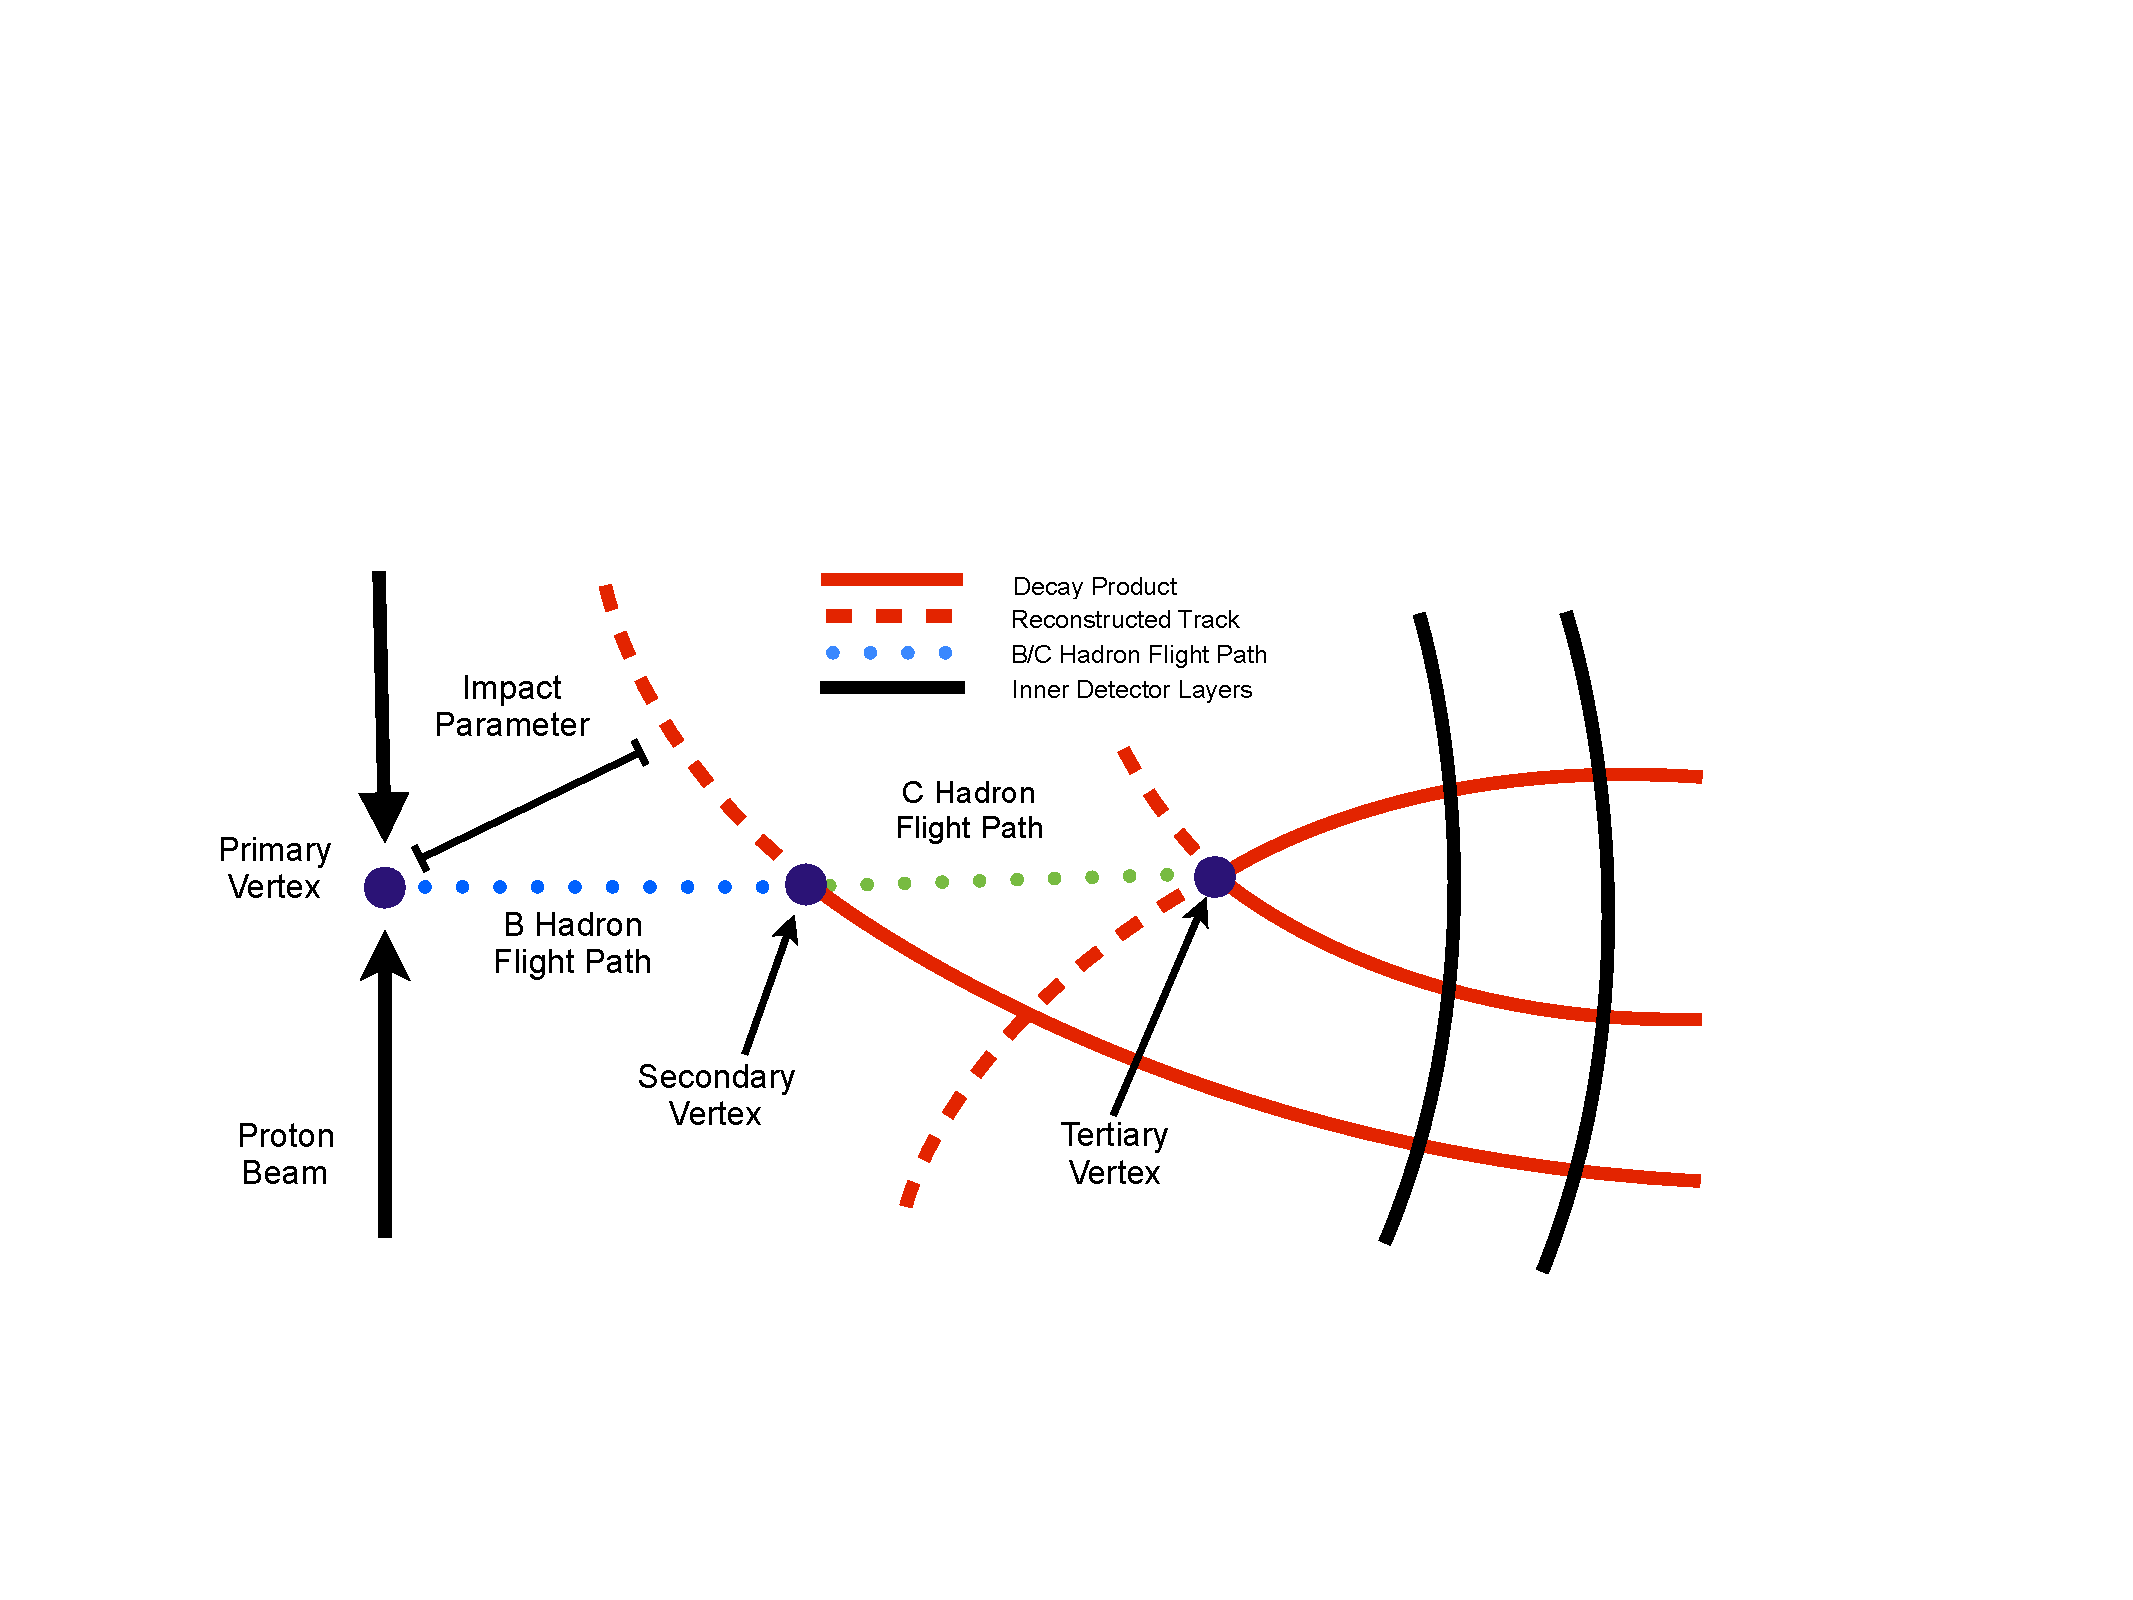
\includegraphics[width=0.9\textwidth]{figs/Objects/bjets_schem.pdf}
    \caption{A diagram to illustrate the key features of a $b$-jet that are utilised by the base $b$-tagging algorithms.}
    \label{fig:obj_bjets_schem}
  \end{center}
  \vspace{-0.5cm}
\end{figure}

\subsubsection{Impact parameter based}
\label{sec:obj-bjets_IP}

The IP3D algorithm is utilises the impact parameter, which is defined as the shortest distance between a specific track and the primary vertex.
A track corresponding to a particle coming from the offset decay vertex of a heavy-hadron is likely to have a large impact parameter,
meaning that the distribution of track impact parameter is different for each of the jet-flavours.
The impact parameter of a track coming from the decay of a heavy hadron is indicated in Figure~\ref{fig:obj_bjets_schem}.
In this algorithm, for all tracks associated to a jet, the impact parameter is calculated in both the transverse (perpendicular to beam-line)
and longitudinal (parallel to beam-line) direction, which are referred to as $d_{0}$ and $z_{0}$.
Then the IP3D algorithm calculates a likelihood of the jet having a specific flavour, 
based on the distributions of the impact parameters ($d_{0}$, $z_{0}$) and their significances 
($d_{0}/\sigma _{d0}$ and  $z_{0}/\sigma_{z0}$) for tracks within the jet. 
Another similar algorithm, IP2D, also calculates the jet flavour likelihood from just the transverse distributions, ($d_{0}$ and $d_{0}$ significance), which is more
robust to pile-up, as tracks from pile-up jets are likely to have a large $z_{0}$ significance value.

\subsubsection{Secondary vertex}
\label{sec:obj-bjets_SV}


The SV1 algorithm aims to reconstruct a secondary vertex of two or more intersecting tracks, corresponding to the decay of a heavy-flavour hadron;
the secondary vertex within a $b$-jet's decay chain is illustrated in Figure~\ref{fig:obj_bjets_schem}.
The SV1 algorithm then calculates many variables that are associated with properties of the reconstructed secondary vertex that show flavour discrimination;
some example variables are the vertex invariant mass,
which will be larger for $b$-jets due to the heavy mass of the $b$-hadron
\footnote{Mass of a B-meson $\sim$ 5 GeV and the mass of a D-meson $\sim$ 1.9 GeV, which are the most common heavy hadrons in a $b$- and $c$-jet respectively.}, 
the distance in the transverse plane between the primary vertex and the secondary vertex, % (2D flight path $L_{XY}$),
which will be larger for $b$-jets due to the long lifetime of the $b$-hadron,
and the number of tracks at the secondary vertex, which will be larger for reliable secondary vertices.

\subsubsection{Jet Fitter}
\label{sec:obj-bjets_JF}

The JetFitter algorithm (JF) attempts to reconstruct the full decay chain of the $b$-hadron into a charmed-hadron and then into light-hadrons. 
This is done by assuming that all vertices lie on a common $b$-flight axis, and then constructing vertices from the intersection of
one or more tracks and the flight axis.
The aim of this is to reconstruct the secondary and tertiary vertices which correspond to the decays of the $b$-hadron and charmed-hadron,
as illustrated in Figure \ref{fig:obj_bjets_schem}.
Similar to SV1, the JetFitter algorithm then calculates a number of flavour discriminating variables:
for example vertex mass and number of vertices with two or more tracks.

\subsubsection{Multi-variate}
\label{sec:obj-bjets_MV2}

The three base algorithms are combined in a boosted decision tree (BDT), a machine-learning technique for combining the many flavour-discriminating variables,
resulting in an algorithm that is known in MV2
As shown in Figure \ref{fig:obj-MV2_schem}, MV2 combines the likelihood output of IP3D and IP2D
with the discriminating variables of SV1 and JF discussed in the preceding sections,
resulting in an output between -1 and 1, where 1 indicates that the jet is likely to be a $b$-jet and -1 indicates the inverse.

\begin{figure}[!htb]
  \begin{center}
    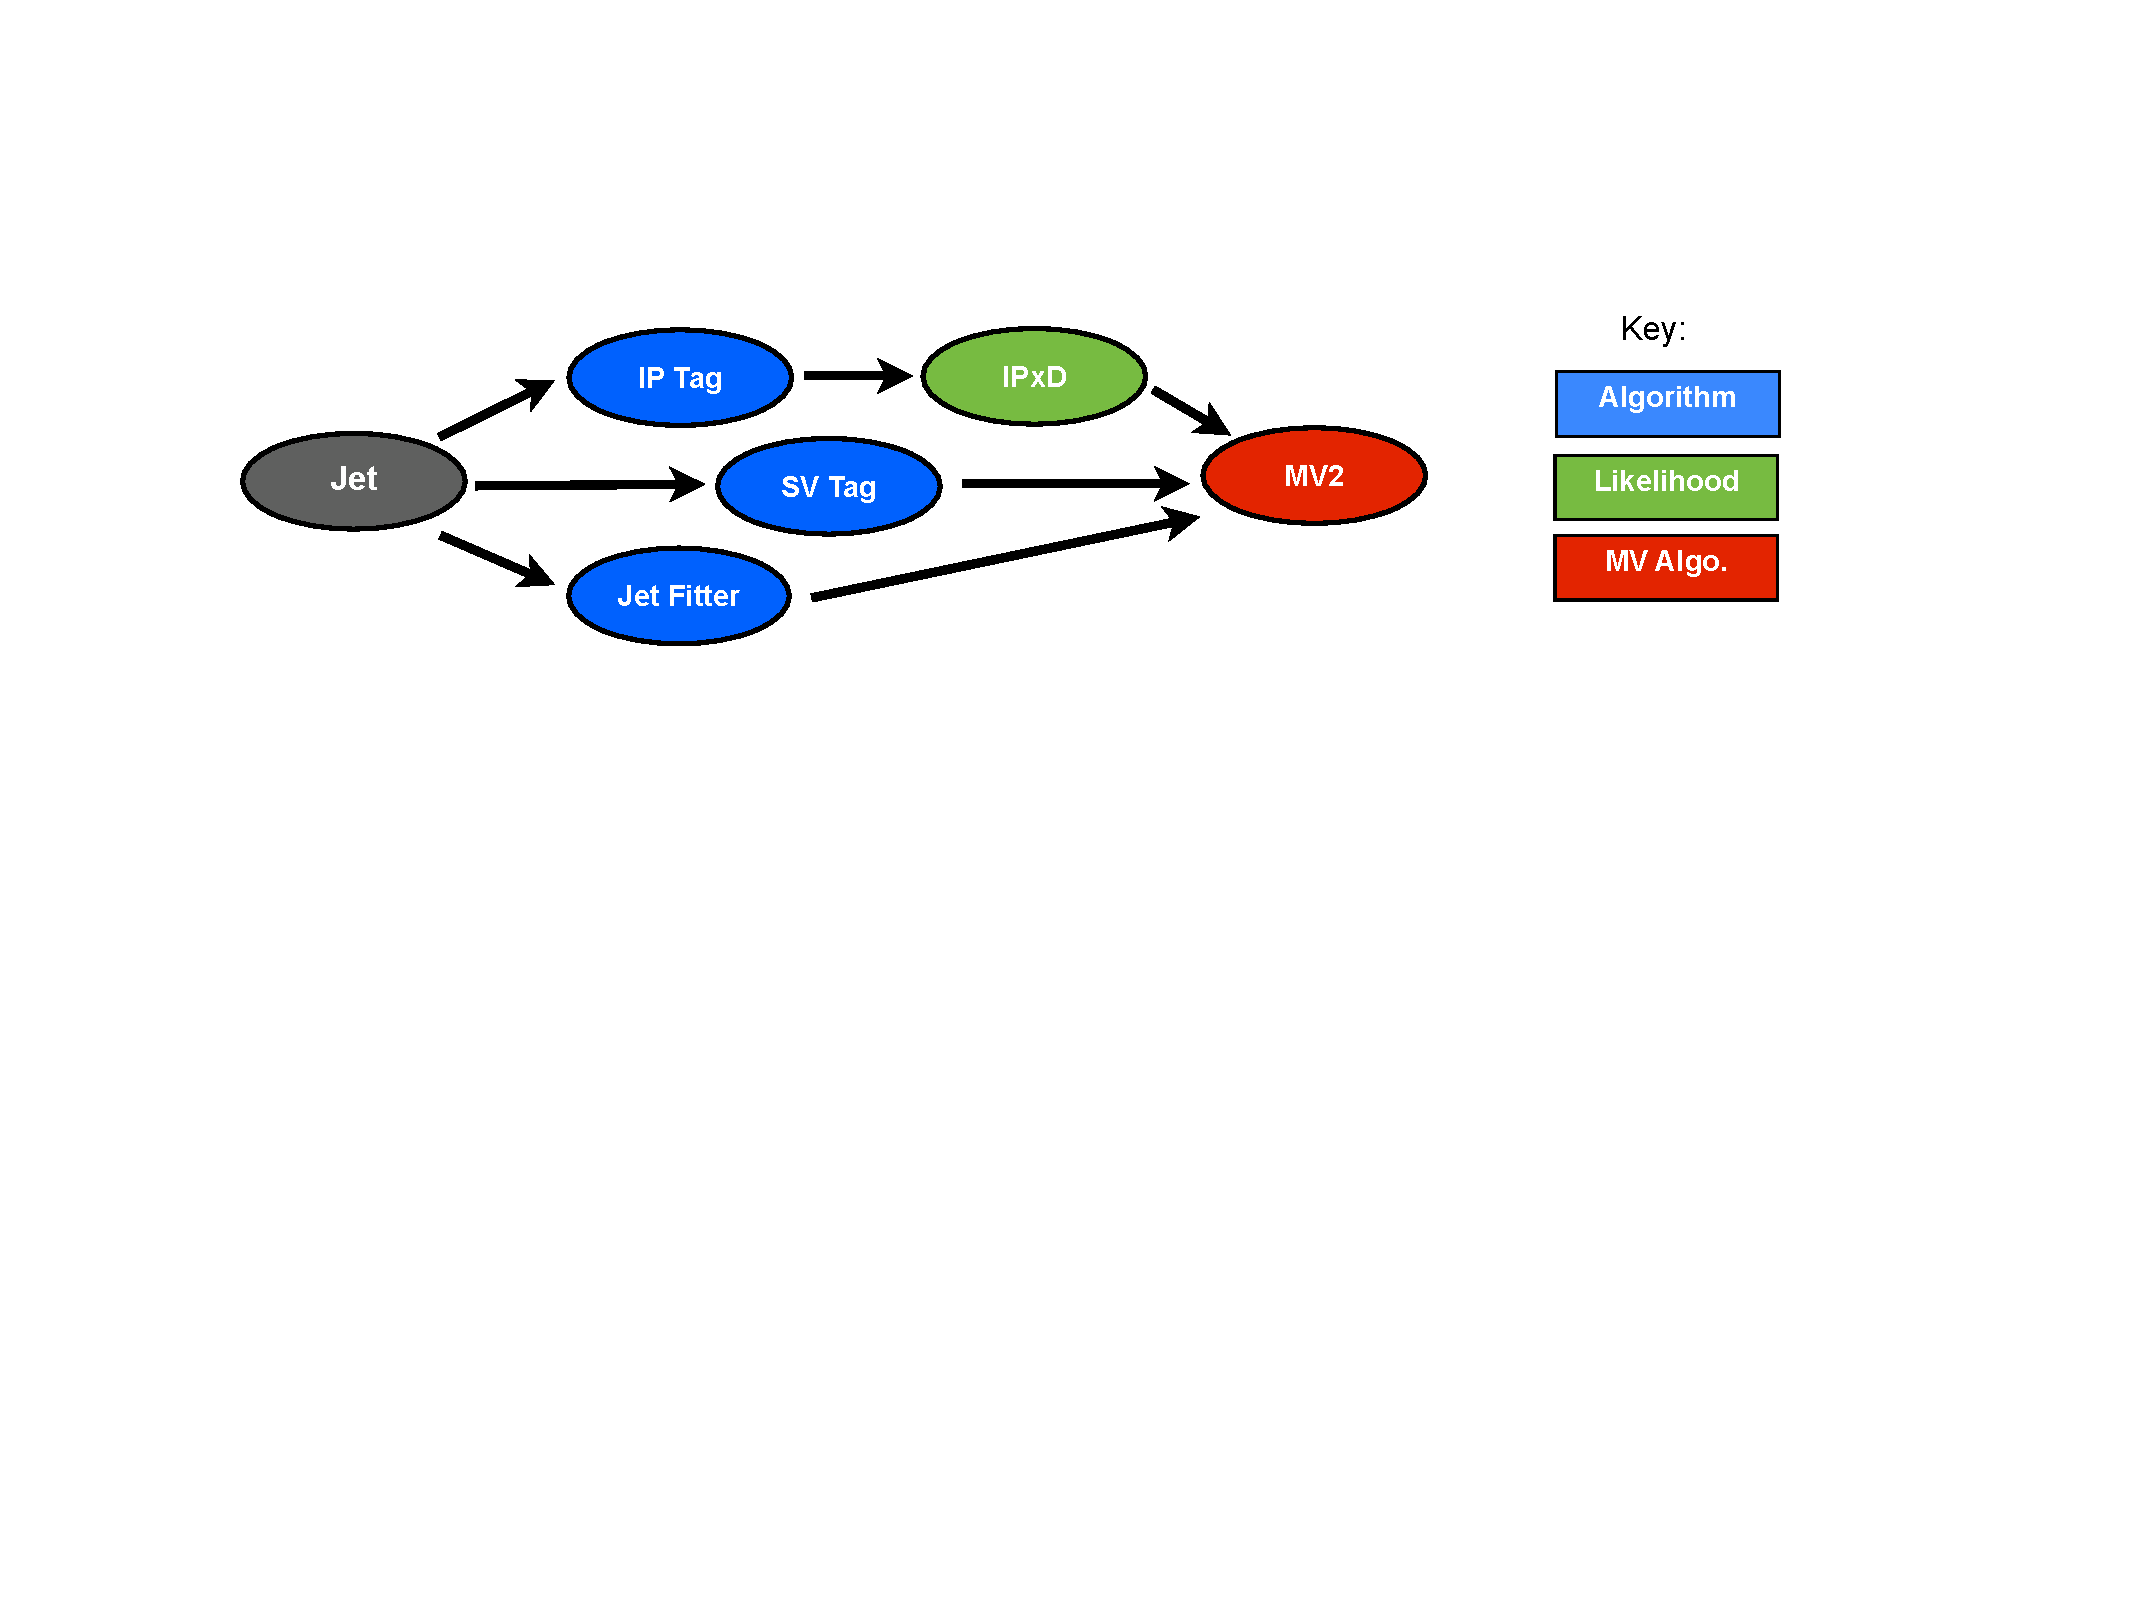
\includegraphics[width=1.0\textwidth]{figs/Objects/MV2_schem.pdf}
    \caption{A diagram illustrating how three base flavour tagging algorithms are combined in the MV2 algorithm.}
    \label{fig:obj-MV2_schem}
  \end{center}
  \vspace{-1cm}
\end{figure}

A cut is then applied to this MV2 output in order to select jets that are likely to $b$-jets.
The cut can be varied to create different operating points which vary the $b$-jet efficiency, light-jet rejection and $c$-jet rejection
\footnote{$b$-jet efficiency is defined as the probability of accepting a true $b$-jet.
  Light-jet rejection is defined as 1 divided by the probability of accepting a true light-jet.
  A similar definition applies for $c$-jet rejection.}.
Looser operating points have a relatively low cut on MV2, meaning that the $b$-jet efficiency is higher at the cost of worse light- and $c$-jet rejections,
and the inverse is true for tighter operating points.
Table~\ref{tab:obj-MV2_WPs} shows the list of fixed cut operating points that are used in ATLAS with a given cut on MV2 output;
shown with the corresponding benchmark $b$-jet efficiency, $c$-jet rejection, light-jet rejection and $\tau$ rejection.
For the remainder of this thesis, the operating points will be referred
\footnote{In this thesis only the fixed-cut operating points shown above will be used,
  however, there also exists a set of flat efficiency operating points where the MV2 cut depends on jet-\pT}
%This is in contrast to the previous multivariate tagger used in Run-1, MV1, which inputted
%the likelihood of a jet having a certain flavour from each of the three base algorithms separately.
\begin{table}[!htb]
  \begin{center}
    \begin{tabular}{|c||c|c|c|c|}
      \hline
      MV2 Cut Value  &  $b$-jet efficiency [\%]  &     $c$-jet rejection   &   Light-jet rejection  &    $\tau$ rejection  \\
      \hline
      0.9349         &           60              &           34          &      1538              &     184              \\
      0.8244         &           70              &           12          &       381              &      55              \\
      0.6459         &           77              &           6           &       134              &      22              \\
      0.1758         &           85              &           3.1         &        33              &     8.2              \\
      \hline
    \end{tabular}
    \caption[The Mv2c10 b-tagging algorithm operating points; with the corresponding $b$-jet~efficiency, $c$-jet~rejection, light-jet~rejection and $\tau$~rejection.]
            {The Mv2c10 b-tagging algorithm operating points; with the corresponding $b$-jet~efficiency, $c$-jet~rejection, light-jet~rejection and $\tau$~rejection.
              This table is taken from reference~\cite{obj-bjets_algo_2016}.}
            \label{fig:obj-MV2_schem}
  \end{center}
  \vspace{-1cm}
\end{table}

The BDT is trained using a simulated sample of $t\bar{t}$ events that will contain a mix of  $b$-, $c$- and light-jets
as well as a sample containing $Z'$ boson decaying to $b$-quarks.
The training makes use of the truth flavour labels assigned to jets using the process described in Section~\ref{sec:obj-bjets_label}.
A training sample with known truth labels is required as this allows the BDT to be optimised
such that it uses the complex correlations between the input variables to allow for high $b$-jet efficiencies
whilst still obtaining a large $c$- and light-jet rejection.
The recommended $b$-tagging tool is MV2c10 which has been trained on a sample containing 10\% charm-jets, to give strong light- and $c$-rejection.

\subsection{Performance}
\label{sec:obj-bjets_calib}

I have a couple of options here.\\
- Put performance in event selection (tagging efficiency plot)\\
- Describe performance here with some discussion of high pT b-Tagging

\section{bTagging: Validation in Dijet Events}

\section{Leptons: Muons and Electrons}   

Reconstruction of electrons and muons is important for a number of analyses at ATLAS;
including the selection of di-lepton $t\bar{t}$ events
which are used in the calibration of $b$-tagging and the $b$-jet trigger,
described in Sections~\label{sec:obj-bjets_calib} and~\label{sec:trig-bjet_eff} respectively.
In addition taus can be identified by the ATLAS detector.
As these objects are not used in the analysis presented in this thesis,
they are described below in less detail than has been given to jets and $b$-jets.

\subsection{Electron}
\label{sec:obj-electron}

Electron reconstruction at ATLAS (which includes positrons) uses
the matching of energy deposits in the calorimeter to
to a track from the inner detector~\cite{obj-electron}.
Information such as the calorimeter shower shape,
properties of the matched track
and TRT transition radiation (described in Section~\ref{sec:det-ID})
allows for identification of electrons with respect to other physics objects described in this section.

\subsection{Muon}
\label{sec:obj-muon}

Muon reconstruction at ATLAS begins uses muon tracks reconstructed using the Muon Spectrometer (MS).
Muon tracks are then extrapolated inwards towards match tracks formed by the Inner Detector (ID).
A global fit is then performed on the combined muon and Inner Detector track,
at which point hits in the MS can be added or removed to improve muon quality.
Muons constructed using this technique are referred to as combined muons
Further details on combined muon reconstruction along with
other muon reconstruction techniques can be found in~\ref{obj-muons}.


